\chapter{Solução}
\label{cap:solucao}

Este capítulo tem por finalidade apresentar a integração entre as tecnologias e ferramentas que fazem parte da solução proposta por este trabalho.

\section{Visão Geral da Solução}
\label{sec:visao-geral}

A solução proposta neste trabalho contempla a utilização de beacon wifi para que os usuários de dispositivos inteligentes, como smartphones, possam ser receber informações em forma de notificação. A figura abaixo demonstra o fluxo e os componentes envolvidos na solução: 

\begin{figure}[h!]
	\centering
	\Caption{\label{fig:visao-geral} Visão Geral}	
	\UECEfig{}{
		\fbox{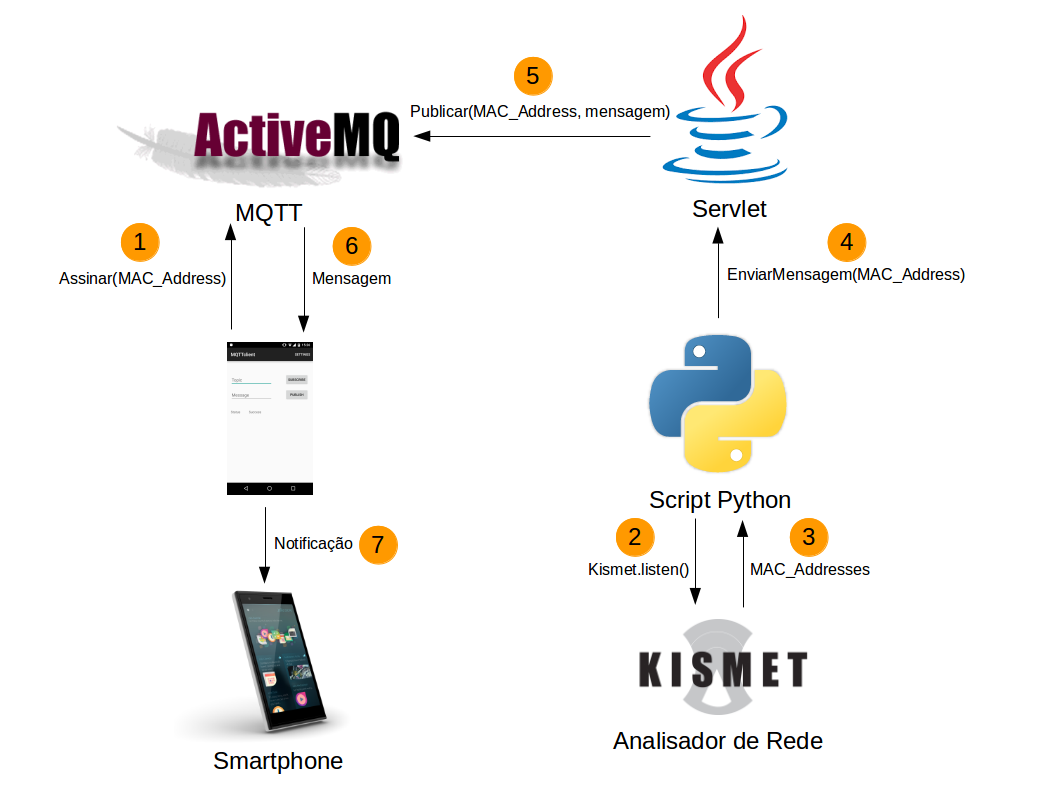
\includegraphics[width=15cm]{figuras/Diagrama-Visao-Geral}}
	}{
	\Fonte{Elaborado pelo autor}			
}	
\end{figure}

\indent O beacon wifi é construído a partir do microcomputador Raspberry Pi contendo o sistema operacional Raspbian instalado juntamente com Kismet, python, TomEE, ActiveMQ e mais duas antenas wifi de conexão usb. Uma antena para detecção dos dispositivos e outra para conexão dos mesmos dispositivos via wifi com o beacon. A conexão via wifi com o beacon poderá ser utilizada tanto para comunicação da aplicação com o agente de mensagens, quanto para compartilhamento de sinal de internet usando um cabo conectado a porta ethernet do Raspberry Pi. \\  
\indent Para que ocorra a detecção dos dispositivos, nesse caso o smartphone, é necessário que os mesmos estejam com o wifi ligado. A detecção fica sob responsabilidade do Kismet, que através da antena wifi em modo de monitoramento capturam os dispositivos com wifi ligado dentro do seu raio de alcance. \\
\indent Uma vez que o dispositivo é detectado, para que as notificações sejam enviadas aos dispositivos, seguindo o protocolo MQTT, é necessária a assinatura de algum tópico de mensagem, o que na solução proposta acontece de forma implícita através da aplicação, que assina um tópico representando o MAC address do dispositivo. Desta forma, é possível identificá-lo de forma única, assim as mensagens poderão conter informações com conteúdo baseado no perfil do usuário do dispositivo. Mas nada impede que o usuário possa também assinar outros tópicos de seu interesse, assim receberá informações categorizadas. Como por exemplo, em uma loja de varejo o usuário receber notificações contendo informação de novos produtos, ofertas ou promoções. \\
\indent O script feito com a linguagem de programação python é responsável por coletar os dados de detecção gerados pelo Kismet através do método kismet.listen(), a medida que os dados são coletados o MAC address é filtrado para em seguida ser enviado pelo script para o servlet que contém o serviço da solução. \\
\indent O serviço, que fica hospedado no servidor de aplicações TomEE, tem como função principal passar as informações a serem enviadas pelo agente de mensagens. Ao receber o MAC address de um dispositivo detectado, o serviço poderá acessar outras fontes de dados, como um banco de dados ou webservice para extrair dados com base na identificação do usuário através do MAC address e formatar mensagens personalizadas para o usuário. Citando novamente o exemplo do uso de beacon em uma loja de varejo, o usuário poderá receber uma notificação contendo recomendações de produtos com base nos últimos produtos comprados por ele. \\
\indent O agente de mensagens utilizado pela solução proposta é o ActiveMQ, configurado para trabalhar internamente usando o protocolo MQTT. É ele de fato quem conhece e entrega as mensagens aos dispositivos. Todas as interações tanto de assinatura, quanto de publicação serão realizadas através do ActiveMQ. Também é possível que outras aplicações de uso administrativo sejam integradas para realizar o gerenciamento dos tópicos de mensagens, assinantes ou até envio direto de mensagem sem intermédio de um serviço. \\
\indent O aplicativo instalado no smartphone do usuário é o responsável por gerar a notificação assim que uma mensagem enviada pelo ActiveMQ é entregue. Mas para que isso ocorra, na aplicação existe um serviço implementado que é iniciado no momento que o dispositivo é ligado, este serviço é gerenciado pelo próprio sistema operacional do smartphone, ficando ativo enquanto o dispositivo permanecer ligado, o que garante que a notificação seja disparada mesmo que o usuário não esteja com a aplicação aberta.

\section{Instalando Raspbian}
\label{sec:instalando-raspbian}

O sistema operacional Raspbian é instalado em um cartão SD comum, sendo recomendado a utilização de cartões com no mínimo 8GB de espaço. O arquivo (zip) de imagem oficial pode ser obtido através do endereço: \\

\url{https://www.raspberrypi.org/downloads/raspbian/} \\

Após baixar o arquivo 2015-09-24-raspbian-jessie.zip (versão atual), o mesmo deve ser descompactado. Para isso o comando abaixo deve ser executado: \\

\begin{lstlisting}[language=bash]
$ unzip Downloads/2015-09-24-raspbian-jessie.zip
\end{lstlisting}

%\begin{lstlisting}[style=BashInputStyle]
%$ apt-get --purge remove rubygems
%\end{lstlisting}

O arquivo resultante será 2015-09-24-raspbian-jessie.img. Para gravar a imagem no cartão SD, o comando abaixo deve ser executado: \\

\begin{lstlisting}[language=bash]
$ dd if=/caminho/ate/imagem of=/dev/sdx
\end{lstlisting}

Onde /caminho/ate/imagem representa literalmente o caminho até onde está a imagem que foi descompactada no comando anterior e /dev/sdx é a particão que representa o cartão SD no sistema operacional.

Por fim, é necessário expandir a partição reservada aos arquivos do sistema Raspbian (ext4) para ocupar todo o espaço restante disponível no cartão SD. Para isso é recomendada a utilização do programa GParted, selecionando a opção de redimensionamento e em seguida alterar o valor do campo ``Novo tamanho (MB)'' para o máximo valor disponível em megabytes. Conforme imagem abaixo:

\begin{figure}[h!]
	\centering
	\Caption{\label{fig:gparted} Expandindo partição com GParted}	
	\UECEfig{}{
		\fbox{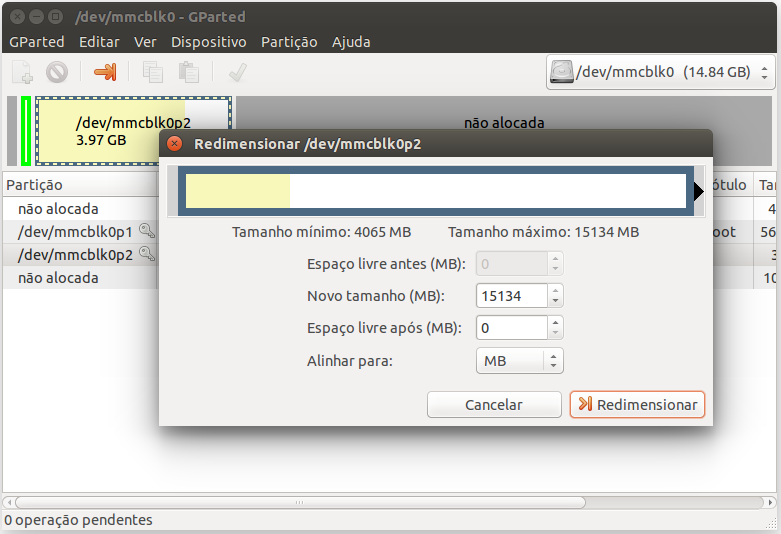
\includegraphics[width=11cm]{figuras/gparted}}
	}{
	\Fonte{Elaborado pelo autor}			
}	
\end{figure}

Após expandir a partição no cartão SD, o sistema estará pronto para ser iniciado.

\begin{figure}[h!]
	\centering
	\Caption{\label{fig:raspbian} Área de trabalho do Raspbian}	
	\UECEfig{}{
		\fbox{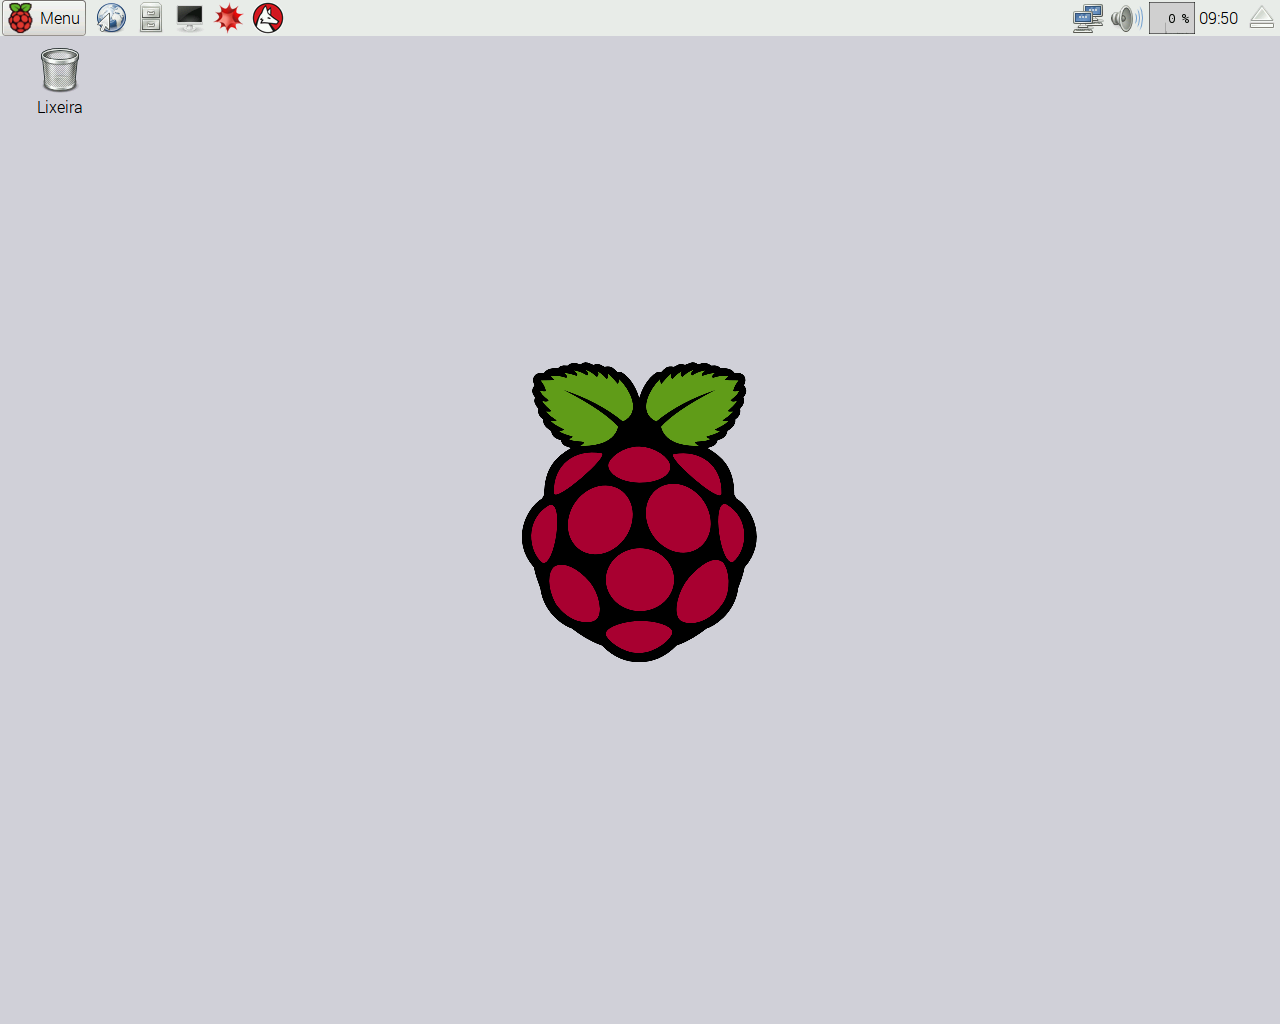
\includegraphics[width=11cm]{figuras/raspbian}}
	}{
	\Fonte{Elaborado pelo autor}			
}	
\end{figure}

Para completar a expansão, a opção ``Expand Filesystem'' no programa de configuração do sistema deve ser utilizada. O programa de configuração está disponível em: Menu>>Preferências>>Raspberry Pi Configuration. Conforme figura abaixo:

\begin{figure}[h!]
	\centering
	\Caption{\label{fig:raspbian} Programa de configuração do Raspbian}	
	\UECEfig{}{
		\fbox{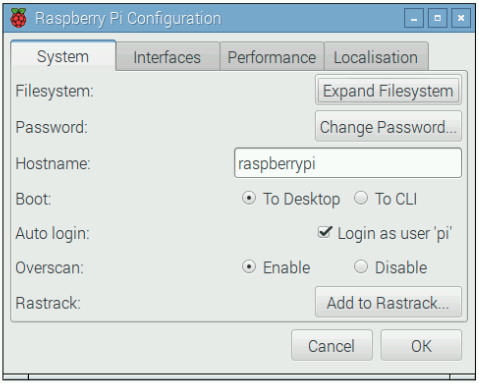
\includegraphics[width=11cm]{figuras/expand}}
	}{
	\Fonte{Elaborado pelo autor}			
}	
\end{figure}

\section{Criando Access Point}
\label{sec:access-point}

Esta seção apresenta todos as ferramentas e configurações necessárias para fazer com que o Raspberry Pi torne-se um ponto de acesso wifi.

O comando abaixo atualiza a lista de pacotes do gerenciador apt-get: \\

\begin{lstlisting}[language=bash]
$ sudo apt-get update
\end{lstlisting}

Após a lista de pacotes ser atualizada, as ferramentas hostapd e isc-dhcp-server poderão ser instaladas executando o comando abaixo. São elas que, de fato, transformam o Raspberry Pi em um ponto de acesso wifi. \\

\begin{lstlisting}[language=bash]
$ sudo apt-get install hostapd isc-dhcp-server
\end{lstlisting}

O hostapd é a ferramenta que implementa as funções de um ponto de acesso no linux e o isc-dhcp-server é o serviço que irá prover os endereços IPs aos dispositivos que conectarem no ponto de acesso.

\subsection{Configurando o ISC DHCP Server}
\label{sec:isc-dhcp-server}

O primeiro arquivo a ser configurado é o dhcpd.conf através do seguinte comando: \\

\begin{lstlisting}[language=bash]
$  sudo nano /etc/dhcp/dhcpd.conf
\end{lstlisting}

No comando acima está sendo utilizado o editor nano, mas outro editor pode ser utilizado. \\
\indent Após o arquivo ser aberto no editor, as seguintes linhas devem ser localizadas: \\

\begin{lstlisting}
option domain-name "example.org";
option domain-name-servers ns1.example.org, ns2.example.org;
\end{lstlisting}

Após localizar, o carácter \# deve ser colocado no início das duas linhas. Como abaixo: \\

\begin{lstlisting}
#option domain-name "example.org";
#option domain-name-servers ns1.example.org, ns2.example.org;
\end{lstlisting}

O próximo passo é localizar as seguintes linhas: \\

\begin{lstlisting}
# If this DHCP server is the official DHCP server for the local
# network, the authoritative directive should be uncommented.
#authoritative;
\end{lstlisting}

Em seguida, o carácter \# deve ser removido da última linha. Ficando como abaixo: \\

\begin{lstlisting}
# If this DHCP server is the official DHCP server for the local
# network, the authoritative directive should be uncommented.
authoritative;
\end{lstlisting}

Feitos os passos anteriores, as seguintes linhas devem ser acrescentadas no final do arquivo dhcpd.conf: \\

\begin{lstlisting}
subnet 10.2.0.0 netmask 255.255.255.0 {
		range 10.2.0.10 10.2.0.50;
		option broadcast-address 10.2.0.255;
		option routers 10.2.0.9;
		default-lease-time 600;
		max-lease-time 7200;
		option domain-name "local";
		option domain-name-servers 8.8.8.8, 8.8.4.4;
}
\end{lstlisting}

As principais configurações definidas nas linhas acima é a sub-rede, máscara de rede e a faixa de IPs a serem distribuídas pelo serviço DHCP. Para salvar todas as configurações realizadas no arquivo dhcpd.conf, deve ser utilizada a combinação de teclas Ctrl+O e para sair do editor Ctrl+X.

O segundo arquivo a ser configurado é o isc-dhcp-server através do seguinte comando: \\

\begin{lstlisting}[language=bash]
$   sudo nano /etc/default/isc-dhcp-server
\end{lstlisting}

Após o arquivo ser aberto no editor, a seguintes linhas devem ser localizadas: \\

\begin{lstlisting}
# On what interfaces should the DHCP server (dhcpd) serve DHCP requests?
#       Separate multiple interfaces with spaces, e.g. "eth0 eth1".
INTERFACES=""
\end{lstlisting}

Após localizar, a última linha deve ser alterada acrescentando a interface wlan0 entre as aspas. Como no exemplo abaixo: \\

\begin{lstlisting}
# On what interfaces should the DHCP server (dhcpd) serve DHCP requests?
#       Separate multiple interfaces with spaces, e.g. "eth0 eth1".
INTERFACES="wlan0"
\end{lstlisting}

Para salvar as configurações realizadas no arquivo isc-dhcp-server, deve ser utilizada novamente a combinação de teclas Ctrl+O e para sair do editor Ctrl+X.

\subsection{Configurando o IP estático para interface wlan0}
\label{sec:ip-estatico-wlan0}

O IP estático deve ser configurado no arquivo interfaces através do comando: \\

\begin{lstlisting}[language=bash]
$   sudo nano /etc/network/interfaces
\end{lstlisting}

Após o arquivo ser aberto no editor, deve ser verificado se já existe qualquer tipo de configuração relacionada a interface wlan0. Caso exista alguma, deve ser removida ou comentada com o carácter \#. Devendo ser mantida somente a linha allow-hotplug wlan0.

Em seguida, devem ser adicionadas as seguintes linhas: \\

\begin{lstlisting}
iface wlan0 inet static
		address 10.2.0.9
		netmask 255.255.255.0 
\end{lstlisting}

As configurações devem ser salvas utilizando a combinação de teclas Ctrl+O e para sair do editor Ctrl+X.

Por fim, o IP estático deve ser associado a interface wlan0 através do comando: \\

\begin{lstlisting}[language=bash]
$   sudo ifconfig wlan0 10.2.0.9
\end{lstlisting}

\subsection{Configurando o hostapd}
\label{sec:configurando-hostapd}

No hostapd são configurados os detalhes do ponto de acesso , como SSID e a senha do ponto de acesso. Para isso, o primeiro passo é criar o arquivo de configuração hostapd.conf na pasta /etc/hostapd. O comando abaixo, utilizando o editor nano, criará o arquivo caso ele não exista: \\

\begin{lstlisting}[language=bash]
$   sudo nano /etc/hostapd/hostapd.conf
\end{lstlisting}

Após isso, já no editor, as linhas seguintes devem ser acrescentadas: \\

\begin{lstlisting}
interface=wlan0
driver=rtl871xdrv
ssid=RPi_AP
hw_mode=g
channel=6
macaddr_acl=0
auth_algs=1
ignore_broadcast_ssid=0
wpa=2
wpa_passphrase=Raspberry123
wpa_key_mgmt=WPA-PSK
wpa_pairwise=TKIP
rsn_pairwise=CCMP 
\end{lstlisting}

Nas linhas de configuração acima, as informações referentes ao ssid e wpa\_passphrase podem ser modificadas conforme necessidade. E o driver deve ser informado de acordo com o modelo do adaptador wifi utilizado.

As configurações devem ser salvas através das combinações de teclas Ctrl+O e Ctrl+X para sair do editor.

O segundo arquivo a ser configurado é o hostapd na pasta /etc/default com o comando abaixo: \\

\begin{lstlisting}[language=bash]
$   sudo nano /etc/default/hostapd
\end{lstlisting}

Após o arquivo ser aberto no editor, a seguinte linha deve ser localizada: \\

\begin{lstlisting}
#DAEMON_CONF="" 
\end{lstlisting}

A linha localizada deve ser modificada retirando o carácter \# e atribuindo entre as aspas o caminho até o arquivo hostapd configurado anteriormente. Conforme abaixo: \\

\begin{lstlisting}
DAEMON_CONF="/etc/hostapd/hostapd.conf"
\end{lstlisting}

Por último, as configurações realizadas devem ser salvas com Ctrl+O e Ctrl+X para sair.

\subsection{Configurando o NAT}
\label{sec:configurando-nat}

NAT é um protocolo que faz a conversão dos endereços IP de uma rede para endereços IP de outra rede. Mas para o contexto deste trabalho, o NAT será utilizado para converter os endereços IP dos dispositivos conectados para um único endereço IP para acesso à internet.

O primeiro arquivo a ser modificado é o sysctl.conf, o mesmo pode ser acessado com o comando abaixo: \\

\begin{lstlisting}[language=bash]
$   sudo nano /etc/sysctl.conf
\end{lstlisting}

Após aberto no editor, a seguinte linha deve ser acrescentada no final do arquivo: \\

\begin{lstlisting}
net.ipv4.ip_forward=1
\end{lstlisting}

A modificação deve ser salva com os comandos Ctrl+O e Ctrl+X.

Para ativar a nova configuração, o seguinte comando deve ser executado: \\

\begin{lstlisting}[language=bash]
$   sudo sh -c "echo 1 > /proc/sys/net/ipv4/ip_forward"
\end{lstlisting}

O próximo passo é configurar a conversão de endereços entre as interfaces eth0 e wlan0 com os comandos abaixo: \\

\begin{lstlisting}[language=bash]
$   sudo iptables -t nat -A POSTROUTING -o eth0 -j MASQUERADE
$   sudo iptables -A FORWARD -i eth0 -o wlan0 -m state --state RELATED,ESTABLISHED -j ACCEPT
$   sudo iptables -A FORWARD -i wlan0 -o eth0 -j ACCEPT
\end{lstlisting}

Para fazer com que os comandos anteriores não precisem ser executados novamente quando o Raspberry Pi for iniciado. O próximo comando deve ser executado: \\

\begin{lstlisting}[language=bash]
$   sudo sh -c "iptables-save > /etc/iptables.ipv4.nat"
\end{lstlisting}

O último arquivo a ser configurado é o interfaces com o seguinte comando: \\

\begin{lstlisting}[language=bash]
$   sudo nano /etc/network/interfaces
\end{lstlisting}

Após aberto no editor, a seguinte linha de ser acrescentada no final do arquivo: \\

\begin{lstlisting}
up iptables-restore < /etc/iptables.ipv4.nat
\end{lstlisting}

A configuração deve ser salva com Ctrl+O e Ctrl+X.

\subsection{Finalizando a Configuração}
\label{sec:finalizando-configuracao}

Nesta seção serão realizadas as últimas configurações do ponto de acesso wifi.

Primeiramente, é necessário iniciar os serviços do hostapd e isc-dhcp-server com os comandos: \\

\begin{lstlisting}[language=bash]
$   sudo service hostapd start 
$   sudo service isc-dhcp-server start
\end{lstlisting}

E por último, para iniciar os serviços sempre que o sistema Raspbian iniciar. Os comandos abaixo devem ser executados: \\

\begin{lstlisting}[language=bash]
$   sudo update-rc.d hostapd enable 
$   sudo update-rc.d isc-dhcp-server enable
\end{lstlisting}

\section{Instalando o Kismet}
\label{sec:instalando-kismet}

O Kismet tem um papel fundamental na solução proposta, pois ele é o responsável por detectar os dispositivos dentro da área de alcance da antena wifi. 

Para baixar e iniciar a instalação do Kismet execute o comando: \\

\begin{lstlisting}[language=bash]
$   sudo apt-get install kismet
\end{lstlisting}

Durante a instalação, será informado que o Kismet necessita de privilégios administrativos para realizar algumas de suas funções, conforme Figura 13. No entanto, executá-lo diretamente como root pode ser algo prejudicial a segurança do sistema. Então é recomendada a instalação com o bit ``setuid'' ativado, assim é permitido a execução de suas funções com os privilégios administrativos garantidos para os processos que tenha essa necessidade.

Ativar o bit ``setuid'' significa permitir que somente usuários adicionados no grupo ``kismet'' possam executar funções como: captura de pacotes de rede e colocar a placa wifi em modo de monitoramento.

\begin{figure}[h!]
	\centering
	\Caption{\label{fig:instalacao_kismet_1} Configuração Kismet - Tela 1}	
	\UECEfig{}{
		\fbox{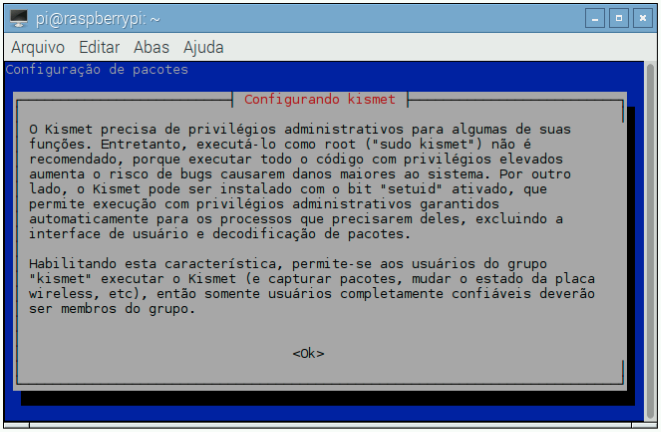
\includegraphics[width=12cm]{figuras/instalacao_kismet_1}}
	}{
	\Fonte{Elaborado pelo autor}			
}	
\end{figure}

Após selecionar a opção <Ok> na tela acima, será questionada a instalação do Kismet com o bit ``setuid'' ativado. Para isso deve ser selecionada a opção <Sim> na tela abaixo:

\begin{figure}[h!]
	\centering
	\Caption{\label{fig:instalacao_kismet_2} Configuração Kismet - Tela 2}	
	\UECEfig{}{
		\fbox{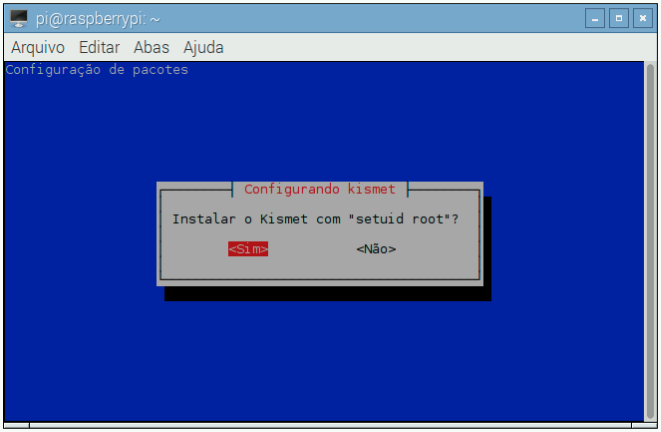
\includegraphics[width=12cm]{figuras/instalacao_kismet_2}}
	}{
	\Fonte{Elaborado pelo autor}			
}	
\end{figure}

Em seguida, os usuários do sistema que irão executar o Kismet devem ser adicionado no grupo ``kismet''. Na próxima tela, o usuário ``pi'' deve ser adicionado no campo texto e confirmado através da opção <Ok>.

\begin{figure}[h!]
	\centering
	\Caption{\label{fig:instalacao_kismet_2} Configuração Kismet - Tela 3}	
	\UECEfig{}{
		\fbox{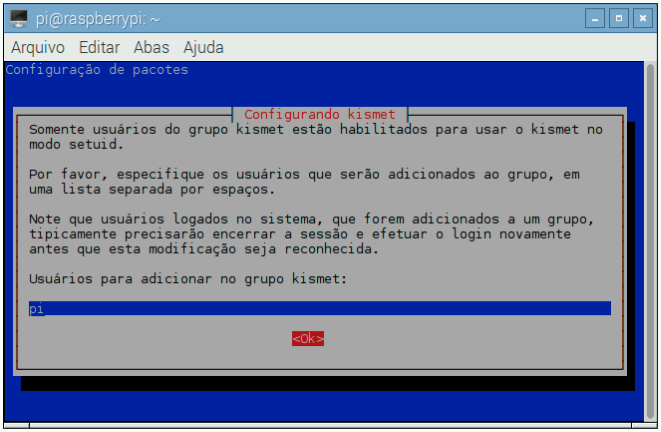
\includegraphics[width=12cm]{figuras/instalacao_kismet_3}}
	}{
	\Fonte{Elaborado pelo autor}			
}	
\end{figure}

Após o término da instalação, o arquivo kismet.conf deverá ser modificado. Para isso o comando abaixo deve ser executado: \\

\begin{lstlisting}[language=bash]
$   sudo nano /etc/kismet/kismet.conf
\end{lstlisting}

Após o arquivo ser aberto no editor, a seguinte linha deve ser localizada: \\

\begin{lstlisting}
gps=true
\end{lstlisting}

E modificada para: \\

\begin{lstlisting}
gps=false
\end{lstlisting}

Em seguida será necessário informar ao Kismet a sua fonte para captura de dados. No caso desta proposta, é a interface wlan1. Para isso deve ser localizada a linha: \\

\begin{lstlisting}
# ncsource=wlan0
\end{lstlisting}

E o carácter ``\#'' deve ser retirado e wlan0 alterado para wlan1: \\

\begin{lstlisting}
ncsource=wlan1
\end{lstlisting}

Após as modificações feitas acima, Ctrl+O para salvar e Ctrl+X para sair do editor.

\section{Script de Detecção}
\label{sec:script-deteccao}

O script de detecção é o componente desta solução que se comunica diretamente com o Kismet para coletar os dados de pacotes capturados pelo analisador. O script é feito na linguagem python e utiliza a biblioteca KismetClient para comunicação com o Kismet Server para obter os dados de captura.

%Para instalar a biblioteca KismetClient no python, é preciso primeiramente instalar o gerenciador de pacotes da linguagem, chamado ``pip''. Para isso deve ser executado o comando abaixo: \\

\subsection{Instalando o KismetClient}
\label{sec:instalando-kismetclient}

A linguagem python já vem instalada por padrão no sistema Raspbian, não necessitando de nenhum comando adicional para seu funcionamento. Então será preciso instalar somente o KismetClient no python, usando o seguinte comando para clonar a biblioteca: \\

\begin{lstlisting}[language=bash]
$   git clone https://github.com/PaulMcMillan/kismetclient.git
\end{lstlisting}

Após clonar a biblioteca, a pasta principal da biblioteca deve ser acessada com o comando: \\

\begin{lstlisting}[language=bash]
$   cd kismetclient/
\end{lstlisting}

Por último, execute o comando para instalar: \\

\begin{lstlisting}[language=bash]
$   sudo python setup.py install
\end{lstlisting}

\subsection{Código do Script}
\label{sec:codigo-script}

O código do script python pode ser criado e editado em qualquer editor de texto, devendo ser salvo sempre com a extensão ``.py''.

No início do script é preciso importar a biblioteca KismetClient com o código abaixo: \\

\begin{lstlisting}[language=python]
from kismetclient import Client as KismetClient
\end{lstlisting}

Logo após, o seguinte código realiza a conexão com o Kismet Server: \\

\begin{lstlisting}[language=python]
address = ('127.0.0.1', 2501)
k = KismetClient(address)
\end{lstlisting}

No código abaixo o protocolo TIME é desativado, pois não é ele que contém as informações dos dispositivos alvos de captura. Em seguida o protocolo CLIENT é ativado especificando os dados relevantes da captura. \\

\begin{lstlisting}[language=python]
k.cmd('REMOVE','TIME')
k.cmd('ENABLE','CLIENT','bssid,mac,signal_dbm,firsttime,lasttime,datapackets')
\end{lstlisting}

O próximo passo é criar e registrar um manipulador customizado de protocolo. É no manipulador que os dados de captura serão recebidos e tratados, como no código abaixo: \\

\begin{lstlisting}[language=python]
def handle_ssid(client, bssid, mac, signal_dbm, firsttime, lasttime, datapackets):
	print 'bssid spotted: {} with mac {} and {} and {} and {} and {}'.format(bssid, mac, signal_dbm, time.strftime("%D %H:%M:%S", time.localtime(int(firsttime))), time.strftime("%D %H:%M:%S", time.localtime(int(lasttime))), datapackets)
	global flag
	if mac == "F8:A9:D0:30:04:63" and flag == False:
		flag = True
		start_new_thread(sendMessage,(mac,))

k.register_handler('CLIENT', handle_ssid)
\end{lstlisting}

Código da função sendMessage utilizada no manipulador: \\

\begin{lstlisting}[language=python]
def sendMessage(topic):
	macAddress = str(topic).replace(":","")
	data = urllib.urlencode({"topic":macAddress, "message":"teste"})
	u = urllib.urlopen("http://10.2.0.9:8080/BeaconServlet/SendMessage?%s" % data)
\end{lstlisting}

E por último, chamar a função listen(): \\

\begin{lstlisting}[language=python]
while True:
	k.listen()
\end{lstlisting}

O método listen() recebe os dados do Kismet Server e encaminha-os para os manipuladores registrados. No código anterior, encaminha para handle\_ssid.

\section{Java Servlet}
\label{sec:java-servlet}

O objetivo do servlet na solução proposta é prover o serviço que recebe os endereços MAC enviados pelo script python, definir a mensagem a ser enviada e encaminhá-la ao agente de mensagens para publicação.

Java Servlets necessitam de um servidor de aplicação para serem acessíveis e executados. O servidor de aplicações que será utilizado neste trabalho é Apache TomEE.

\subsection{Instalando o Apache TomEE}
\label{sec:instalando-tomee}

O arquivo para instalação do Apache TomEE está disponível em: \\

\begin{lstlisting}
http://tomee.apache.org/downloads.html
\end{lstlisting}

A versão do TomEE utilizada neste trabalho é a plume. Por se tratar da versão mais completa em termos de recursos.

Após baixar o arquivo, execute o seguinte comando para descompatar e ao mesmo tempo mover a pasta descompactada para os arquivos do sistema na pasta opt: \\

\begin{lstlisting}[language=bash]
$   sudo tar -zxvf apache-tomee-1.7.2-plume.tar.gz && mv apache-tomee-plume-1.7.2 /opt/
\end{lstlisting}

Em seguida deve ser criado e configurado um shell script para inicialização do TomEE durante a inicialização do sistema Raspbian.

Execute o comando abaixo para criar um arquivo chamado tomee-plume na pasta init.d do sistema: \\

\begin{lstlisting}[language=bash]
$   sudo nano /etc/init.d/tomee-plume
\end{lstlisting}

No editor, o código abaixo deve ser redigido: \\ 

\begin{lstlisting}[language=bash,caption={bash version}]
#!/bin/sh
# Tomee-Plume Init-Script

case $1 in

start)
sh /opt/apache-tomee-plume-1.7.2/bin/startup.sh
;;

stop)
sh /opt/apache-tomee-plume-1.7.2/bin/shutdown.sh
;;

restart)
sh /opt/apache-tomee-plume-1.7.2/bin/shutdown.sh
sh /opt/apache-tomee-plume-1.7.2/bin/startup.sh
;;

esac

exit 0
\end{lstlisting}

Após o código ser salvo, é preciso executar o seguinte comando para atribuir permissão ao arquivo: \\

\begin{lstlisting}[language=bash]
$   sudo chmod 755 /etc/init.d/tomee-plume
\end{lstlisting}

Logo após atribuir a permissão, o comando abaixo precisa ser executado para que o gerenciador de scripts ``update-rc.d'' possa reconhecer o script tomee-plume. \\

\begin{lstlisting}[language=bash]
$   sudo update-rc.d tomee-plume defaults
\end{lstlisting}

E por último, executar o seguinte comando para iniciar o Apache TomEE: \\

\begin{lstlisting}[language=bash]
$   /etc/init.d/tomee-plume start
\end{lstlisting}

\subsection{Configurando o TomEE}
\label{sec:configurando-tomee}

Para que o Apache TomEE possa comunicar com o agente de mensagens é preciso configurar o arquivo tomee.xml localizado na pasta conf.

Para isso, o seguinte comando deve ser executado: \\

\begin{lstlisting}[language=bash]
$   sudo nano /opt/apache-tomee-plume-1.7.2/conf/tomee.xml
\end{lstlisting}

A tag abaixo deve ser localizada: \\

\begin{lstlisting}[language=xml]
<tomee>
	...
</tomee>
\end{lstlisting}

E as seguintes tags ``Resource'' devem ser incluídas: \\

\begin{lstlisting}[language=xml]
<tomee>
	<Resource id="MyJmsResourceAdapter" type="ActiveMQResourceAdapter">
		BrokerXmlConfig =
		ServerUrl       =  tcp://someHostName:61616
	</Resource>

	<Resource id="MyJmsConnectionFactory" type="javax.jms.ConnectionFactory">
		ResourceAdapter = MyJmsResourceAdapter
	</Resource>
</tomee>
\end{lstlisting}

\subsection{Código do Servlet}
\label{sec:codigo-servlet}

O código do servlet pode variar muito dependendo da forma como os dados que compõe a mensagem serão obtidos e formatados para o usuário. Seja através de uma conexão a algum banco de dados ou consumindo webservices. Mas independente disso, o código responsável pelo envio das mensagens para o agente de mensagens sempre segue o mesmo padrão. Como será descrito abaixo:

Primeiro devemos criar uma classe estendendo a classe HttpServlet. Conforme abaixo: \\

\begin{lstlisting}[language=java]
@WebServlet("/SendMessage")
public class SendMessage extends HttpServlet {
	...
}
\end{lstlisting}

E na mesma classe, declarar a conexão: \\

\begin{lstlisting}[language=java]
@WebServlet("/SendMessage")
public class SendMessage extends HttpServlet {

	@Resource
	private ConnectionFactory connectionFactory;
	...
}
\end{lstlisting}

No método doGet ou doPost -- o uso de um ou outro vai depender da necessidade -- deve conter o código responsável pelo envio das mensagens.

O primeiro passo é armazenar os parâmetros enviados pela requisição de envio feita pelo script python. Como a seguir: \\   

\begin{lstlisting}[language=java]
@Override
protected void doGet(HttpServletRequest req, HttpServletResponse resp) throws ServletException, IOException {
	String paramTopic = req.getParameter("topic");
	String paramMessage = req.getParameter("message");
	...
}
\end{lstlisting}

Em seguida a conexão deve ser criada e iniciada: \\

\begin{lstlisting}[language=java]
try {
	Connection connection = connectionFactory.createConnection();

	connection.start();
	...
} catch (JMSException e) {
	e.printStackTrace();
}
\end{lstlisting}

Logo após, uma sessão deve ser criada: \\

\begin{lstlisting}[language=java]
try {
	...
	// Create a Session
	Session session = connection.createSession(false, Session.AUTO_ACKNOWLEDGE);
	...
} catch (JMSException e) {
	e.printStackTrace();
}
\end{lstlisting}

Após criar a sessão, tópico e mensagem são criados: \\ 

\begin{lstlisting}[language=java]
try {
	...
	Topic topic = session.createTopic(paramTopic);

	// Create a MessageProducer from the Session to the Topic or Queue
	MessageProducer producer = session.createProducer(topic);
	producer.setDeliveryMode(DeliveryMode.NON_PERSISTENT);

	// Create a message
	TextMessage message = session.createTextMessage(paramMessage);
	...
} catch (JMSException e) {
	e.printStackTrace();
}
\end{lstlisting}

E por último, a mensagem é enviada: \\

\begin{lstlisting}[language=java]
try {
	...
	// Tell the producer to send the message
	producer.send(message);
} catch (JMSException e) {
	e.printStackTrace();
}
\end{lstlisting}

\section{Agente de Mensagens}
\label{sec:agente-mensagens}

O agente de mensagens utilizado neste trabalho é o ActiveMQ, além de ser de código aberto, o mesmo já tem suporte interno ao protocolo MQTT.

\subsection{Instalação do ActiveMQ}
\label{sec:instalacao-activemq}

Para baixar o arquivo compactado de instalação do ActiveMQ, o seguinte endereço deve ser acessado: \\

\begin{lstlisting}
http://activemq.apache.org/activemq-5121-release.html
\end{lstlisting}

Após baixar o arquivo, o seguinte comando deve ser executado para descompactar e mover o arquivo para pasta opt: \\

\begin{lstlisting}[language=bash]
$   sudo tar -zxvf apache-activemq-5.12.1-bin.tar.gz && mv apache-activemq-5.12.1 /opt/
\end{lstlisting}

Em seguida, deve ser criado um link do arquivo shell script do ActiveMQ para pasta init.d do sistema: \\

\begin{lstlisting}[language=bash]
$   sudo ln -sf /opt/apache-activemq-5.12.1/bin/activemq /etc/init.d/activemq
\end{lstlisting}

Para registrar o arquivo no gerenciador de scripts do sistema, o comando abaixo deve ser executado: \\

\begin{lstlisting}[language=bash]
$   sudo update-rc.d activemq defaults
\end{lstlisting}

Para iniciar o ActiveMQ, o seguinte comando deve ser executado: \\
 
\begin{lstlisting}[language=bash]
$   /etc/init.d/activemq start
\end{lstlisting}

\subsection{Configuração do ActiveMQ}
\label{sec:configuracao-activemq}

Para fazer com que o ActiveMQ funcione com base no protocolo MQTT é preciso alterar o arquivo de configuração.

O arquivo activemq.xml deve ser aberto com o seguinte comando: \\

\begin{lstlisting}[language=bash]
$   sudo nano /opt/apache-activemq-5.12.1/conf/activemq.xml
\end{lstlisting}

No editor, a seguinte tag deve ser localizada: \\

\begin{lstlisting}[language=xml]
<transportConnectors>
	...
</transportConnectors>
\end{lstlisting}

Uma vez localizada, a tag abaixo deve ser incluída: \\

\begin{lstlisting}[language=xml]
<transportConnectors>
	...
	<transportConnector name="mqtt" uri="mqtt://0.0.0.0:1883"/>
	...
</transportConnectors>
\end{lstlisting}

\section{Aplicativo Android}
\label{sec:aplicativo-android}